\section{Methods}

This study integrated naturalistic story-listening fMRI, standardized behavioral assessments and computational language modelling to examine contextual language processing in Cantonese-speaking children (Figure~\ref{fig:fig1_workflow}). The imaging cohort comprised 23 children, including 16 who completed the full literacy, oral-language and cognitive assessment battery. Following preprocessing and quality assessment, BOLD responses were aligned with contextual embeddings and predictive features extracted from Gemma 3 1B. Two complementary analyses characterized the relationship between these model-derived representations and neural responses. A joint voxelwise general linear model estimated signed associations with surprisal, predictive entropy and semantic update, conditional on the other features. Contextual-embedding encoding models used nested leave-one-subject-out cross-validation to evaluate prediction of the 16 assessment-complete children's responses to the same story. Both approaches accounted for speech-related, acoustic and nuisance variation. Selected-voxel summaries were then derived within cortical and subcortical regions defined by the Schaefer--Tian parcellation. With the child as the unit of inference, permutation analyses assessed regional text-feature responses and associations of regional encoding performance and text-feature coefficients with behavioral scores. False discovery rate correction was applied across regions within each predefined family of tests.

\begin{figure}[t]
\centering
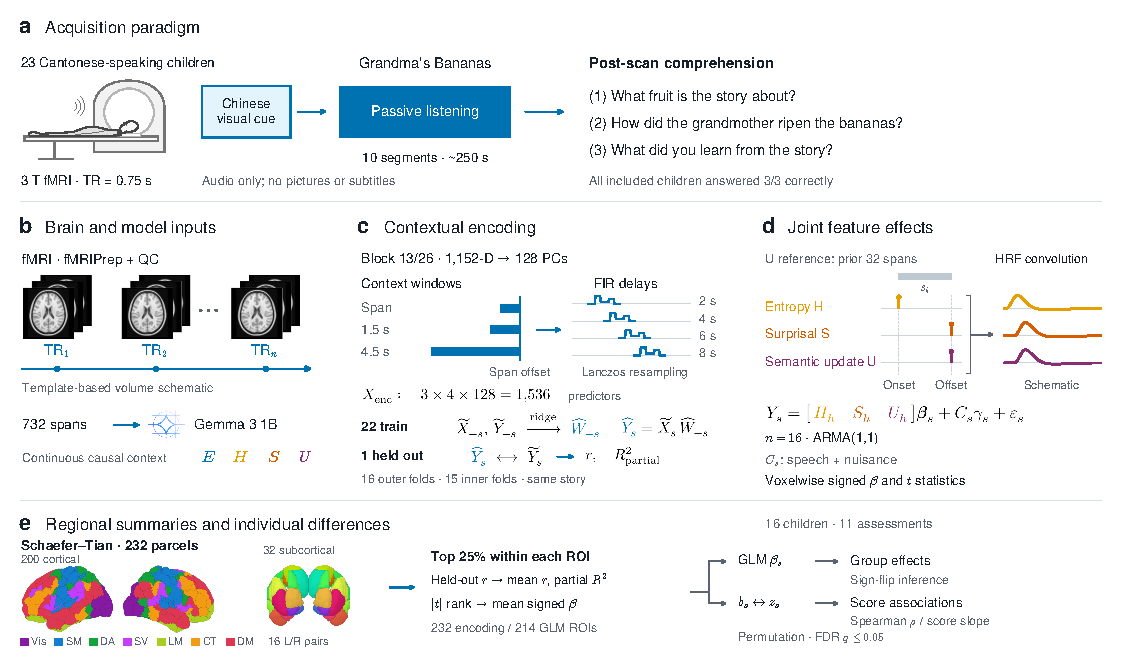
\includegraphics[width=\linewidth]{figures/fig1.pdf}
\caption{\textbf{Naturalistic story-listening paradigm and analysis framework.} \textbf{a}, Cantonese-speaking children listened to a story during fMRI and completed post-scan comprehension questions. \textbf{b}, Story-aligned BOLD preprocessing and extraction of contextual embeddings and predictive features from Gemma 3 1B. MRI thumbnails schematically illustrate volume sampling using a public MNI152NLin6Asym anatomical template. \textbf{c}, Nested leave-one-subject-out encoding linked contextual embeddings to held-out responses; tildes denote nuisance-adjusted quantities. \textbf{d}, A joint voxelwise model estimated signed associations with surprisal, predictive entropy and semantic update. Single-span event curves illustrate haemodynamic convolution, and $C_s$ denotes speech-related and nuisance regressors. \textbf{e}, Atlas-based regional summaries supported group-response and brain--behavior analyses using permutation inference and ROI-wise false discovery rate correction. Atlas colours identify cortical networks and subcortical subdivisions.}
\label{fig:fig1_workflow}
\end{figure}

\subsection{Data acquisition}



\subsubsection{Participants}
Participants were recruited from an ongoing cross-sectional study that included structural and functional MRI and formal assessments of general intelligence, literacy, and language development. All participants spoke Cantonese as their native, dominant, and family language, and attended local mainstream primary schools in Hong Kong where the curriculum was delivered in Cantonese. All children used English as a second language (reported mean age of acquisition [AoA] = 3.45 years) and learned Mandarin at school (reported mean AoA = 5.35 years). In addition, four of the 23 included participants reported learning experience with additional foreign languages, including French, Japanese, and Spanish. The study was approved by the Human Research Committee at The Hong Kong Polytechnic University, and written consent was obtained from each participant and their parent or legal guardian.

Five children were excluded for excessive head motion during scanning, and two were excluded because they fell asleep during scanning. The resulting story-imaging cohort comprised 23 children (12 girls and 11 boys, mean age = 10.59 years, SD = 1.56, range = 7.83–13.17 years).

Of these 23 children, 16 completed the full literacy and language assessments and constituted the brain–behavior cohort. These 16 children also served as held-out participants in the encoding-model evaluation, while the remaining seven contributed training data in every cross-validation fold (Supplementary Fig.~\ref{fig:cohort}). The brain–behavior cohort comprised eight girls and eight boys in grades 2–6 (mean age = 10.24 years, SD = 1.31, range = 8.42–12.25 years; Table~\ref{tab:sample}).

\begin{table}[htbp]\centering\small
\caption{Characteristics of the assessment cohort. All summaries refer to the 16 children used for brain--behavior analyses.}\label{tab:sample}
\begin{tabular}{lrr}\toprule Characteristic & Mean (SD) or count & Range \\\midrule
Age (years) & 10.24 (1.31) & 8.42--12.25 \\
Sex (female/male) & 8/8 & --- \\
School grade & 3.94 (1.39) & 2--6 \\\midrule
Full-scale IQ & 101.50 (11.62) & 85--128 \\
Literacy & 7.64 (3.26) & 1.75--13 \\
Word reading & 8.12 (3.77) & 1--15 \\
Word dictation & 6.31 (3.14) & 1--11 \\
Cantonese grammar & 11.75 (2.35) & 7--14 \\
Discourse comprehension & 11.31 (3.03) & 7--17 \\
Word definition & 12.12 (3.26) & 5--16 \\
Semantic relations & 8.50 (3.41) & 1--13 \\
Story retelling & 9.44 (3.14) & 1--14 \\
Noun expression & 9.88 (3.84) & 1--15 \\
HKGCNT & -0.74 (1.99) & -5.07--1.57 \\
\bottomrule\end{tabular}
\par\smallskip\begin{minipage}{.94\linewidth}\footnotesize Assessment values are the standardized scores supplied in the study assessment table. Age is derived from the recorded mean scan-month age.\end{minipage}
\end{table}

\subsubsection{MRI acquisition}
Whole-brain images were acquired on a 3.0-T Siemens Prisma scanner at The Hong Kong Polytechnic University. Functional data were acquired using an accelerated BOLD echo-planar imaging sequence (EPI; posterior-to-anterior phase encoding). The sequence comprised 60 interleaved slices with 2.4-mm isotropic voxels, a field of view of 216 × 216 mm, repetition time (TR) of 750 ms, echo time (TE) of 30 ms, and flip angle of 60°. A high-resolution T1-weighted structural image was acquired using a sagittal 3D MPRAGE sequence (240 slices; 0.8-mm isotropic voxels; field of view 256 × 224 mm; TR = 2300 ms; TE = 2.07 ms; inversion time = 1100 ms; flip angle = 7°; GRAPPA acceleration factor = 2).

\subsubsection{Story-listening paradigm}
Participants passively listened to a short story during fMRI scanning. A sound check was performed inside the scanner, during which the experimenter adjusted playback volume to each participant’s preferred comfortable level. A brief starting cue ("the story is about to start") was visually presented in Chinese on the screen before narration began.  The auditory-only presentation used Cantonese narration delivered in a soft female voice. The recording comprised ten audio segments lasting approximately 4 min 10 s in total.

The story, ``婆婆嘅香蕉'' (``Grandma's Bananas''), is classified as Level 4 in the Chinese Storybooks collection (https://global-asp.github.io/storybooks-chinese/), which assigns stories to five levels based on length and vocabulary. It follows a child narrator who discovers the grandmother’s secret banana-ripening method, takes bananas, and eventually learns not to steal bananas from the grandmother. The familiar family setting, concrete events, and relatively straightforward narrative sequence make the story appropriate for Cantonese-speaking pupils across Hong Kong Primary 2–6.

After scanning, all participants reported that this was their first exposure to the story. They were also asked three post-scan questions in Cantonese to assess story comprehension: (1) What fruit is the story about? (2) How did the grandmother ripen the bananas? and (3) What did you learn from the story? Only participants who answered all three comprehension questions correctly were included in the sample.

\subsubsection{Literacy, language, and cognitive assessment}
In Hong Kong, locally developed, standardized, norm-referenced assessment batteries are well established for evaluating both Chinese literacy \cite{ho2015hong} and Cantonese spoken language \cite{t2006hong} in school-age children. In clinical and educational practice, these instruments are routinely used to profile language and literacy development and to support the diagnosis of specific learning disorder and developmental language disorder. As they yield age-normed standard scores calibrated to local Hong Kong reference populations, these tools allow for direct, developmentally fair comparisons of individual language and literacy proficiency across primary school age groups.

Literacy was assessed using the Hong Kong Test of Specific Learning Difficulties in Reading and Writing for Primary School Students, Third Edition (HKT-P(III)). Chinese Word Reading and Chinese Word Dictation were the literacy tasks shared across the junior- and senior-primary batteries. These tasks and the overall General Literacy score were included in the analyses. Tables and figures label them word reading, word dictation and literacy, respectively. Scores are reported on the test’s norm-referenced scale (mean = 10, SD = 3); scores of 7 or below were taken to indicate weakness. The HKT-P(III) has Hong Kong norms for children aged 6 years 1 month to 12 years 6 months \cite{ho2015hong}.

Cantonese oral-language ability was assessed using the Hong Kong Cantonese Oral Language Assessment Scale (HKCOLAS). The six subtests were Hong Kong Cantonese Grammar, Textual Comprehension, Word Definition, Lexical-Semantic Relations, Narrative, and Expressive Nominal Vocabulary. The corresponding analysis labels are Cantonese grammar, discourse comprehension, word definition, semantic relations, story retelling and noun expression. HKCOLAS is a norm-referenced assessment developed for Cantonese-speaking children in Hong Kong and standardized on 1,120 children aged 5–12 years. Subtest scores are reported on a scale with a mean of 10 and SD of 3; a score of 10 corresponds to the 50th percentile, and scores of 7 or below indicate weakness \cite{t2006hong}.

General intellectual ability was assessed using the Hong Kong version of the Wechsler Intelligence Scale for Children—Fourth Edition (WISC-IV(HK)). The WISC-IV assesses verbal comprehension, perceptual reasoning, working memory and processing speed, and provides a full-scale IQ index of general intellectual ability \cite{wechsler2010hong}. 

As an additional measure of reading, participants completed the Hong Kong Graded Character Naming Test (HKGCNT). This test assesses oral reading of single Chinese characters of graded difficulty and covers primary grades 1–6 \cite{leung2008hong,mcleod2012multilingual}. The HKGCNT score used in the analyses followed the scoring metric specified in the test manual.

Qualified practitioners administered the assessment and reported the results under the study’s Hong Kong assessment protocol. Registered educational psychologist administered the HKT-P(III) and WISC-IV(HK), while registered speech therapist administered the HKCOLAS and HKGCNT. 

\subsection{MRI preprocessing and quality assessment}
Imaging data were organized according to the Brain Imaging Data Structure (BIDS) \cite{bids} and preprocessed using fMRIPrep version 25.2.7 \cite{fmriprep}. T1-weighted images underwent intensity non-uniformity correction with N4BiasFieldCorrection in ANTs 2.6.2, brain extraction using an OASIS template, and segmentation into grey matter, white matter and cerebrospinal fluid with FSL FAST. FreeSurfer 7.3.2 was used for cortical surface reconstruction and refinement of the anatomical brain mask. Anatomical images were registered nonlinearly to standard space using ANTs.

For each functional run, fMRIPrep generated a blood-oxygen-level-dependent (BOLD) reference image and estimated six rigid-body head-motion parameters with FSL MCFLIRT. Susceptibility distortion correction used the anatomically constrained, fieldmap-less SyN workflow, with deformation restricted to the phase-encoding direction. The BOLD reference was aligned to the T1-weighted image using six-degree-of-freedom boundary-based registration. Slice timing was corrected with AFNI 3dTshift to the beginning of each repetition time (TR). Motion, distortion and spatial-registration transforms were composed for single-step volumetric resampling using cubic B-spline interpolation. The analyses used BOLD images in MNI152NLin6Asym space at 2-mm isotropic resolution.

Quality assessment included visual review of anatomical normalization, BOLD-to-anatomical alignment, coverage and artefacts in the fMRIPrep HTML reports. Quantitative checks assessed sequence length, framewise displacement (FD), standardized DVARS and temporal signal-to-noise ratio. Each selected story run contained 336 volumes at a TR of 0.75 s. Frames were flagged when FD exceeded 0.5 mm, standardized DVARS exceeded 1.5, or fMRIPrep identified a non-steady-state volume \cite{power}. The original acquisition-time grid was retained for stimulus alignment. Flagged frames were represented by individual spike regressors in the text-feature GLM; encoding fitting and performance scoring used the unflagged rows of this same time grid.

Before statistical modelling, BOLD images were spatially smoothed with a 4-mm full-width-at-half-maximum Gaussian kernel normalized within each child's effective brain mask. Voxel time series were expressed as percent signal change (PSC), using the mean signal across unflagged frames as the reference. Common analysis masks were constructed by intersecting the effective masks of the 23 story runs. The encoding mask contained 224,757 voxels and the text-feature GLM mask contained 224,756 voxels.

\subsection{Language model and stimulus-aligned representations}
All reported analyses used Gemma 3 1B (\texttt{google/gemma-3-1b-pt}), the Schaefer--Tian parcellation and the top 25\% of voxels within each ROI; encoding used 128 principal components (PC128). Model parameters and the fixed checkpoint revision are provided in Supplementary Table~\ref{tab:selected_parameters}. Feature extraction used the model's native tokenizer and continuous causal text context.

Character-level annotations provided timing for 869 characters. A common segmentation of 732 contiguous text spans linked these annotations to model features. Each span inherited the onset of its first character and the offset of its final character. Contextual embeddings were extracted at the final token of the exact text prefix ending at each span, from decoder block 13 of 26. Each embedding contained 1,152 dimensions. Prefixes crossing native tokenization boundaries were separately tokenized and evaluated at their own boundaries. This procedure aligned representations with the annotated spans while retaining native tokenization.

Three scalar features described the story's model-derived predictive and contextual dynamics. For span $i$, surprisal was the sum of native token surprisals assigned to that span,
\begin{equation}
 S_i=-\sum_{k\in\mathcal{T}_i}\log_2 P(w_k\mid w_{<k}),
\end{equation}
where $\mathcal{T}_i$ contains tokens whose final character falls within span $i$. Each token contributed once, at the offset of the corresponding common span. Predictive entropy quantified the uncertainty of the native next-token distribution conditional on the text preceding span onset,
\begin{equation}
 H_i=-\sum_{w\in\mathcal{V}}P(w\mid c_i)\log_2 P(w\mid c_i),
\end{equation}
where $\mathcal{V}$ is the model vocabulary and $c_i$ is the exact preceding text prefix.

Semantic update quantified the change in the direction of a recent contextual representation after incorporating the current span. Let $\mathbf{u}_i$ denote the L2-normalized contextual embedding. The preceding context and its update were defined as
\begin{equation}
 \mathbf{m}_i=\frac{1}{32}\sum_{j=i-32}^{i-1}\mathbf{u}_j,
 \qquad
 \mathbf{m}_i^{+}=\frac{32\mathbf{m}_i+\mathbf{u}_i}{33},
 \qquad
 U_i=1-\frac{\mathbf{m}_i^{\mathsf T}\mathbf{m}_i^{+}}
 {\|\mathbf{m}_i\|\,\|\mathbf{m}_i^{+}\|}.
\end{equation}
Semantic update was evaluated from span 33 onward, providing a complete preceding 32-span context for each analysed event.

\subsection{Voxelwise text-feature GLM}
For each child, surprisal, entropy and semantic update were entered jointly into a voxelwise general linear model (GLM). Feature amplitudes were standardized across spans 33--732. Entropy events were placed at span onsets; surprisal and semantic-update events were placed at span offsets. Event trains were convolved with a peak-normalized canonical double-gamma haemodynamic response function (HRF), comprising gamma components with shape parameters 6 and 16 and a 6:1 peak-to-undershoot weighting. The text GLM used 316 BOLD volumes beginning at 15.0 s, the first sampled time point at or after the onset of span 33.

The model included four speech-related control regressors: span-event density, span duration, span token count and the audio root-mean-square envelope. The envelope was calculated in 20-ms windows from audio sampled at 16 kHz. Speech control regressors were HRF-convolved. Motion regressors comprised six parameters, their first derivatives, and the squares of both sets, yielding 24 motion terms. Additional nuisance terms included mean white-matter and cerebrospinal-fluid signals, discrete cosine drift regressors with a 128-s high-pass period, frame-specific spike regressors and an intercept. Thus, each text-feature coefficient estimated the response associated with that feature conditional on the other text features and nuisance terms.

Models were fitted with AFNI 3dREMLfit using voxelwise autoregressive moving-average ARMA(1,1) temporal-noise modelling and generalized least squares\cite{afni,arma}. The outputs included signed PSC coefficients and corresponding $t$ statistics for each of the three text features. The 16 first-level fits yielded 48 feature-specific coefficient maps.

\subsection{Contextual-embedding encoding models}
Encoding models predicted voxelwise BOLD responses from the first 128 principal components of the Gemma 3 1B contextual embeddings. Principal component analysis was fitted to the centred 732-span embedding matrix of the story; these components retained 91.97\% of its variance (Supplementary Table~\ref{tab:selected_parameters}).

To incorporate multiple scales of preceding context, three embedding series were constructed: the current span embedding and the mean embeddings within trailing 1.5-s and 4.5-s windows ending at each span offset. Each series was resampled to fMRI time points with a three-lobe Lanczos filter and expanded with finite impulse response (FIR) delays of 2, 4, 6 and 8 s. For span offset $o_i$, BOLD sampling time $t$ and delay $\ell$, the interpolation weight was
\begin{equation}
 L(u)=\operatorname{sinc}(u)\operatorname{sinc}(u/3)\,
       \mathbb{I}(|u|<3)\mathbb{I}(o_i\leq t),
 \qquad u=\frac{t-\ell-o_i}{\mathrm{TR}},
\end{equation}
with $\operatorname{sinc}(u)=\sin(\pi u)/(\pi u)$. Combining the three context scales and four delays produced 12 feature blocks and 1,536 expanded columns. Each expanded column was centred and scaled across the 324 retained sampling times, beginning at 9.0 s and ending at 251.25 s. An exact singular-value reparameterization expressed the design in its nonzero temporal subspace while preserving the expanded feature kernel and ridge penalty.

BOLD and stimulus predictors were projected into each child's nuisance-residual space using the four speech controls, 24 motion terms, white-matter and cerebrospinal-fluid signals, cosine drifts and intercept. The projection was estimated on that child's unflagged frames. Voxelwise ridge coefficients minimized
\begin{equation}
 \widehat{\boldsymbol{\beta}}_v
 =\arg\min_{\boldsymbol{\beta}}
 \left\{\frac{1}{N_{\mathrm{train}}}
 \sum_{s\in\mathcal{S}_{\mathrm{train}}}
 \|\widetilde{\mathbf y}_{sv}-\widetilde{\mathbf X}_s\boldsymbol{\beta}\|^2
 +\alpha\|\boldsymbol{\beta}\|^2\right\},
\end{equation}
where $N_{\mathrm{train}}$ is the total number of unflagged training frames and tildes denote nuisance-adjusted quantities. Candidate regularization strengths were $\{10^{-3},10^{-2},\ldots,10^{4}\}$.

Nested leave-one-subject-out (LOSO) cross-validation produced predictions for each of the 16 children with complete assessments. Each outer fold trained on the other 22 children. Regularization was selected separately for each voxel by minimizing summed squared error across 15 inner validation folds. Each inner fold withheld one remaining child with complete assessments. The seven additional children contributed to every training fold. Models were then refitted on all 22 outer-fold training children and evaluated on the held-out child's response to the same story.

Two metrics summarized each held-out voxel. Pearson's $r$ measured correspondence between predicted and measured nuisance-adjusted BOLD. Incremental prediction relative to the nuisance baseline was expressed as cross-validated partial $R^2$,
\begin{equation}
 R^2_{\mathrm{partial},v}
 =1-\frac{\sum_{t\in\mathcal{G}_s}(\widetilde y_{svt}-\widehat{\widetilde y}_{svt})^2}
 {\sum_{t\in\mathcal{G}_s}\widetilde y_{svt}^{\,2}}
 =\frac{\mathrm{SSE}_{\mathrm{nuisance}}-\mathrm{SSE}_{\mathrm{full}}}
 {\mathrm{SSE}_{\mathrm{nuisance}}},
\end{equation}
where $\mathcal{G}_s$ denotes the held-out child's unflagged frames. Both measures were carried forward at their observed signed values.

\subsection{Whole-brain parcellation and regional summaries}
Regional analyses used Schaefer's 200-region cortical atlas combined with the 32-region Tian scale-2 subcortical atlas \cite{schaefer,tian}. Atlas labels were aligned with the common 2-mm analysis grid. Encoding analyses included all 232 represented regions. Text-feature GLM analyses required at least 80\% of a region's atlas voxels to fall within the common mask, yielding 214 eligible regions.

Within each region of interest (ROI), the top 25\% of covered voxels were summarized. The selected count was the ceiling of 0.25 multiplied by the number of covered ROI voxels. For text GLMs, voxels were ranked separately for each child and feature by the absolute first-level $t$ statistic; the signed coefficients of the selected voxels were then averaged. For encoding models, voxels were ranked by that child's held-out Pearson correlation, and the selected voxels' $r$ and partial $R^2$ values were averaged arithmetically. Voxel selection used each child's imaging statistic; assessment scores entered the subsequent association analysis.

Encoding performance maps show the arithmetic mean of each regional summary across the 16 held-out children. Atlas-wide descriptive summaries gave equal weight to the 232 ROIs within each child. The mean and sample SD were then calculated across children. Source data provide each regional mean and SD.

Regional values were displayed on the inflated fsaverage cortical surface (10,242 vertices per hemisphere). MNI152 atlas labels were projected using registration-fusion coordinates distributed with neuromaps \cite{neuromaps}. Nearest-neighbour sampling preserved discrete parcel identities during projection onto the surface. Values were assigned to the corresponding surface parcels and the medial wall was masked. Left and right lateral and medial views used fixed camera positions. Text-feature group maps display BH-FDR-significant cortical results with direct ROI names and a common signed $t$ scale; subcortical results appear in named statistic matrices. Brain--behavior location maps identify the ROI and association direction, with adjacent individual-level scatterplots and effect summaries. Scatterplots include descriptive ordinary least-squares lines with pointwise 95\% Student's $t$ confidence bands for the fitted mean. Marginal Gaussian kernel-density estimates use Scott bandwidths and are displayed over the observed value ranges, with rug marks for individual observations. All regional estimation and inference used the original volumetric analysis grid.

\subsection{Regional inference and multiple-comparison correction}
The child was the unit of inference. Text-feature group responses were assessed with an intercept-only second-level model of the 16 children's regional coefficients. Two-sided permutation probabilities were obtained from all 32,768 distinct sign-pattern representatives after accounting for equivalence of opposite signs. Assessment associations were estimated separately for each score using
\begin{equation}
 \overline{\beta}_{sr}=a_r+b_r z_s+\epsilon_{sr},
\end{equation}
where $\overline{\beta}_{sr}$ is the child's selected-voxel regional coefficient and $z_s$ is the assessment score centred and scaled by its sample SD. The slope $b_r$ expresses the change in regional coefficient per SD of assessment score. Two-sided score-permutation probabilities used 19,999 random permutations plus the observed assignment. Analytic 95\% confidence intervals for group means and slopes were computed with the corresponding Student's $t$ distribution.

Encoding--assessment associations were quantified with Spearman's rank correlation across the 16 children. Exact two-sided probabilities were computed from the full label-permutation distribution using a dynamic-programming calculation of rank-dot-product counts. Tied ranks were assigned their average values, and the permutation distribution retained the multiplicity of individual label assignments.

The Benjamini--Hochberg false discovery rate (BH-FDR) procedure \cite{bh} was applied at $q\leq0.05$. Each text-GLM family comprised the 214 eligible ROIs for one text feature and one group or individual-assessment contrast. Each encoding family comprised the 232 ROIs for one performance metric and one assessment. Group-response and brain--behavior plots display results passing these ROI-wise thresholds. Each significant assessment association is accompanied by the corresponding individual participant values. Encoding-performance panels display descriptive cross-validated estimates. Supplementary Table~\ref{tab:counts} reports the complete test totals for this specification; source data provide regional estimates and probabilities.

